\documentclass{article}
\usepackage{hyperref}
\usepackage{graphicx}
\usepackage{float}
\begin{document}
\title{Sensors for FRC}

\author{SoftwareBug2.0, Team 1425}
\date{\today}

\maketitle

\tableofcontents

\section{Introduction}

for each type:
theory of operation
output results \& accuracy/what it measures
example use
selection criteria \& different types
programming schemes
reliability
	-failure modes
		-environmental
		-detectability
		-non-environmental
wiring
cost, availablity
power use
weight

types known to be used on FIRST robots

\section{Limit switches and bump sensors}

\begin{figure}[ht]
\centering
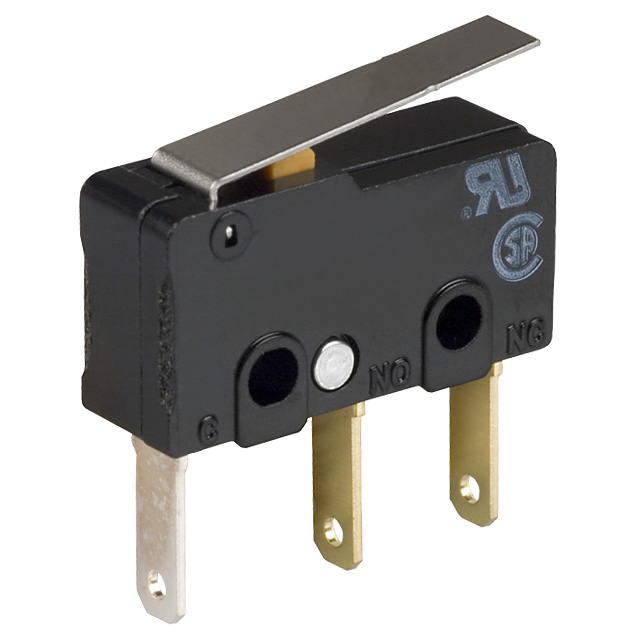
\includegraphics[width=2in]{Spdt_limit_switch.jpg}
\caption{Typical limit switch}
\end{figure}

\begin{figure}[ht]
\centering
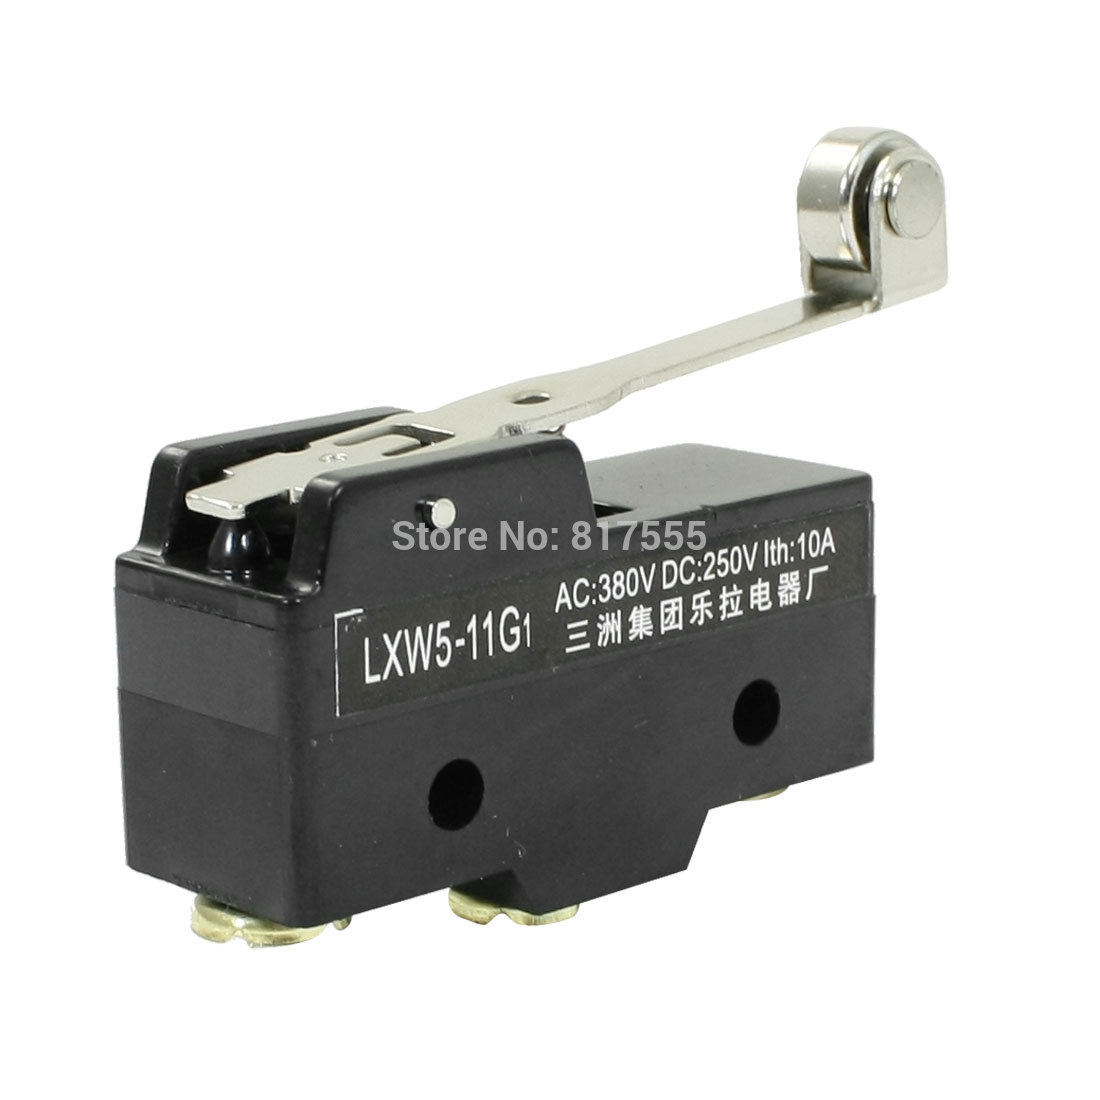
\includegraphics[width=2in]{limit_wheel.jpg}
\caption{Limit switch with roller}
\end{figure}

\begin{figure}[ht]
\centering
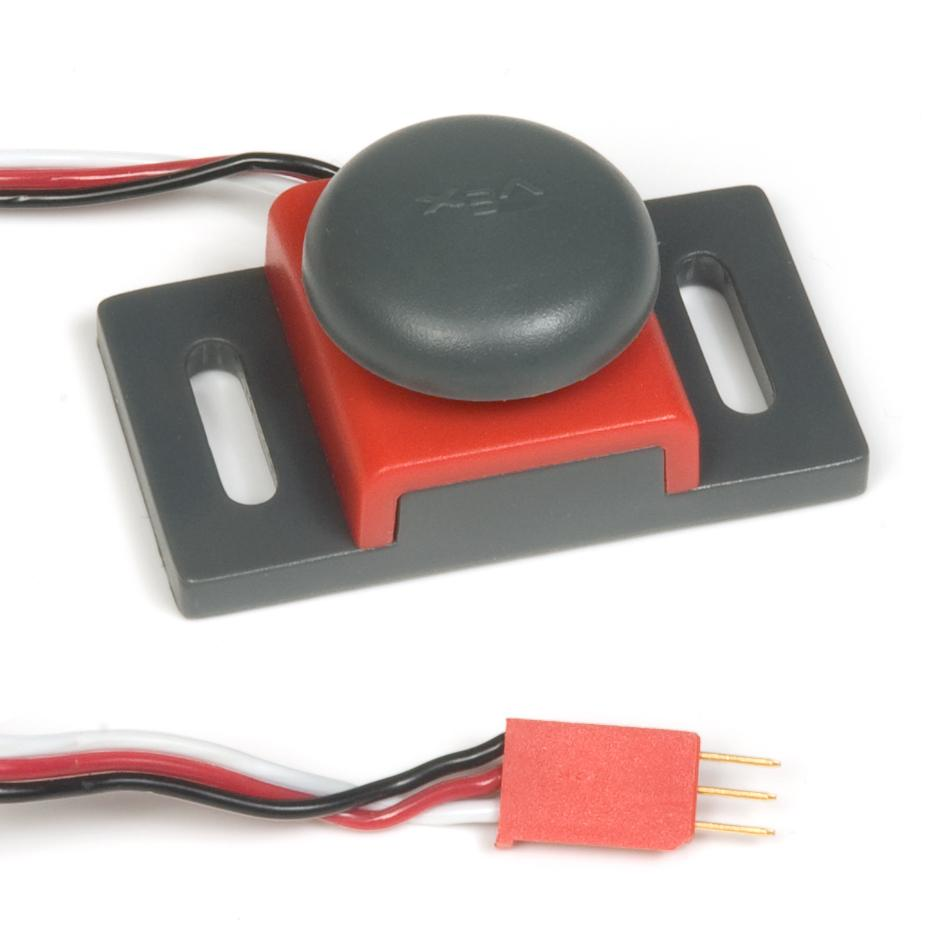
\includegraphics[width=2in]{vex_switch.jpg}
\caption{Vex-brand bump sensor}
\end{figure}

Limit switches and bumb sensors work by physically opening and closing a connection between two sets of contacts.  They produce a binary output and tend to have good repeatability of when they change states.  We used some of these on our 2004 robot to stop an arm extension when it was at either end.  

The major differentiating factor between these switches is their physical package.  Pick the one that can be mounted well and is least likely to become physically broken in a given application.  

These would typically be wired to a digital IO with an extra resistor soldered somewhere.  These types of switches are widely available (always in stock at Fry's) and many switches of this types are not more than a couple dollars.  When properly wired they should have negligible energy use and should weigh under an ounce.  

\section{Hall-effect sensors}
Hall effect sensors detect magnets.  They are often used like a Use like a limit switch or like an encoder on high-speed stuff

\section{Magnetic cylinder sensors}
These clamp on to the side of a pneumatic cylinder and if the right kind of cylinder then it goes ahead and tries to make it so that it has a magnet inside near the end of the piston

\section{Encoders}

\begin{figure}[ht]
\centering
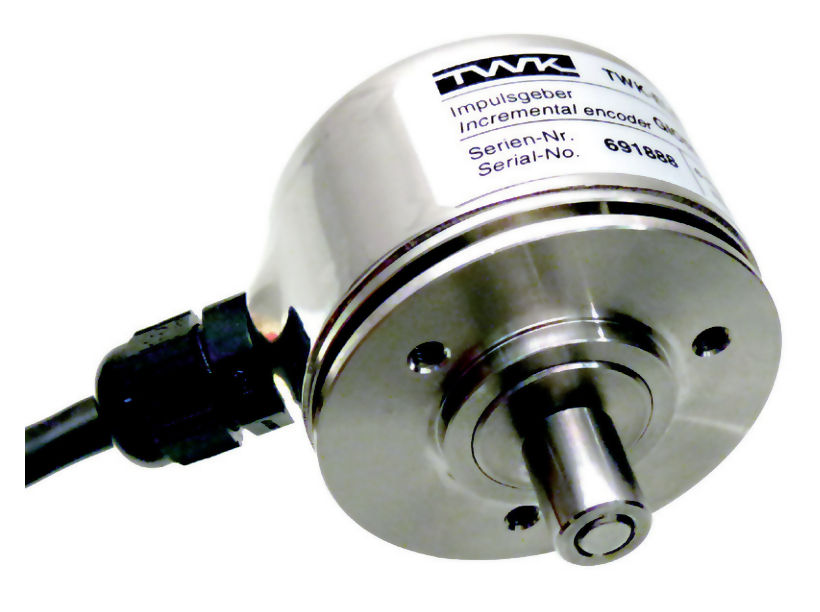
\includegraphics[width=2in]{encoder_shaft.jpg}
\caption{Encoder with integrated shaft}
\end{figure}

\begin{figure}[ht]
\centering
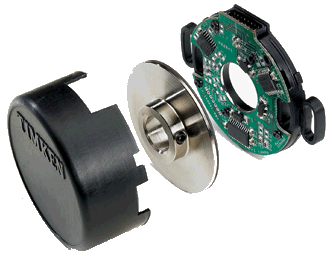
\includegraphics[width=2in]{encoder_slip.png}
\caption{Enc1oder which slips onto a shaft}
\end{figure}

number of counts
\section{Potentiometers}
\begin{figure}[ht]
\centering
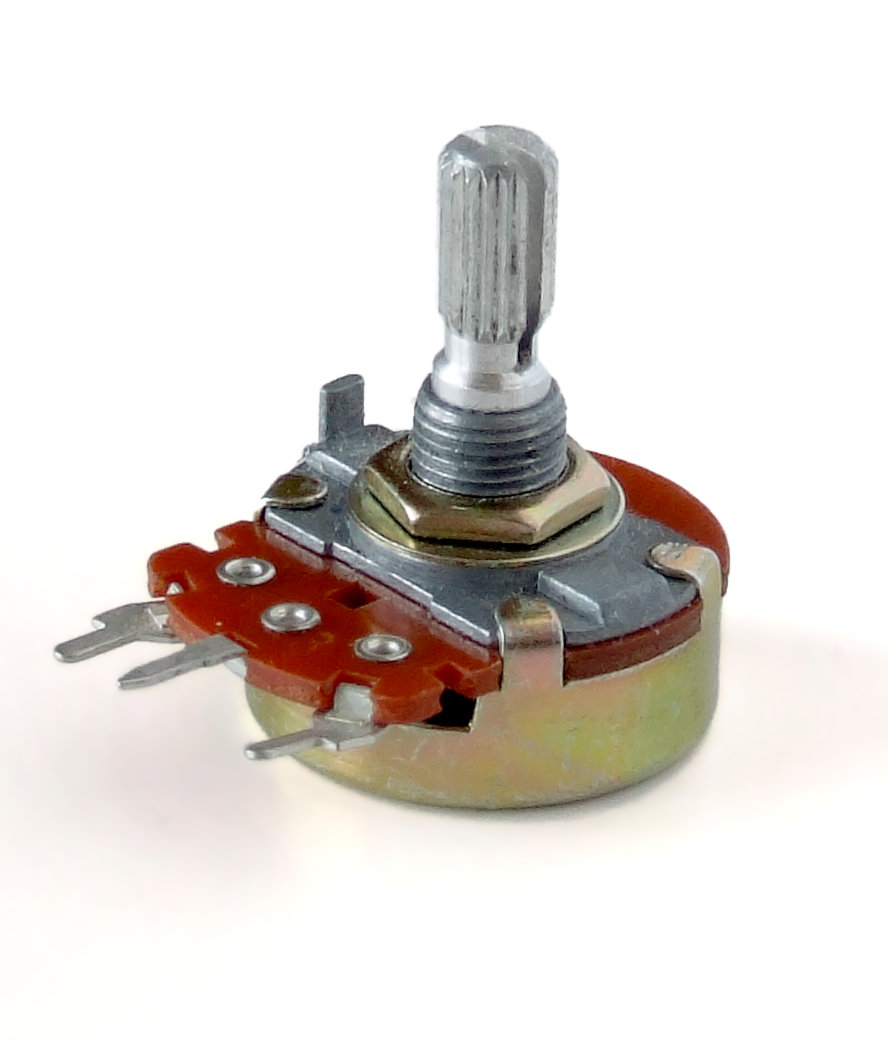
\includegraphics[width=2in]{Potentiometer.jpg}
\caption{Potentiometer.  The shaft that extends vertically rotates.}
\end{figure}

\section{Current sensing}
\begin{figure}[ht]
\centering
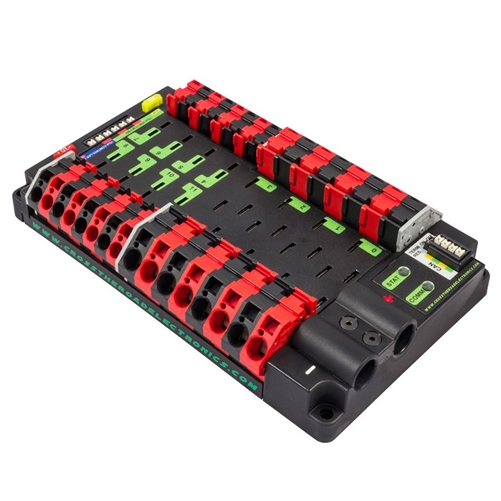
\includegraphics[width=2in]{pdp.jpg}
\caption{The power distribution panel contains built-in current sensing for each output.}
\end{figure}

\section{Accelerometers}
\begin{figure}[ht]
\centering
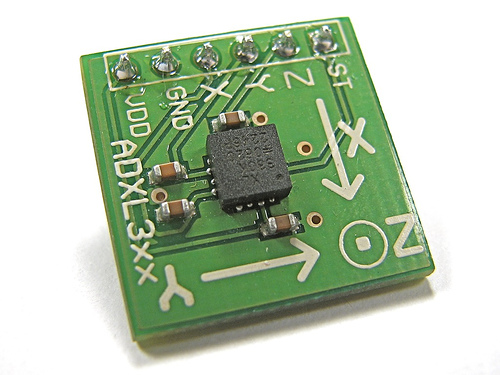
\includegraphics[width=2in]{accelerometer.jpg}
\caption{A breakout board with axes labeled.  The black chip in the center is the accelerometer itself.}
\end{figure}

\begin{figure}[ht]
\centering
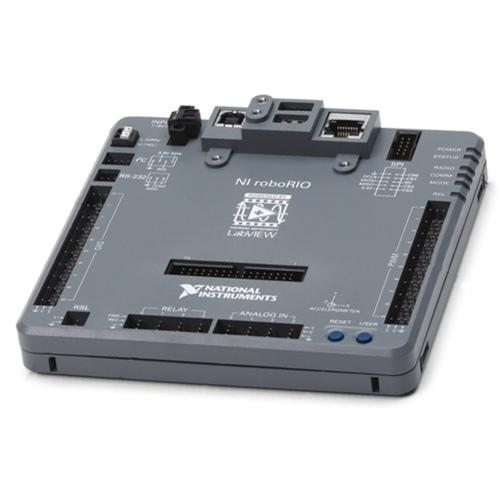
\includegraphics[width=2in]{roborio.jpg}
\caption{The roboRIO contains a built-in three-axis accelerometer.}
\end{figure}

Tilt sensor
Integration \& drift
\section{Gyros}


\section{Ultrasonic}
\begin{figure}[ht]
\centering
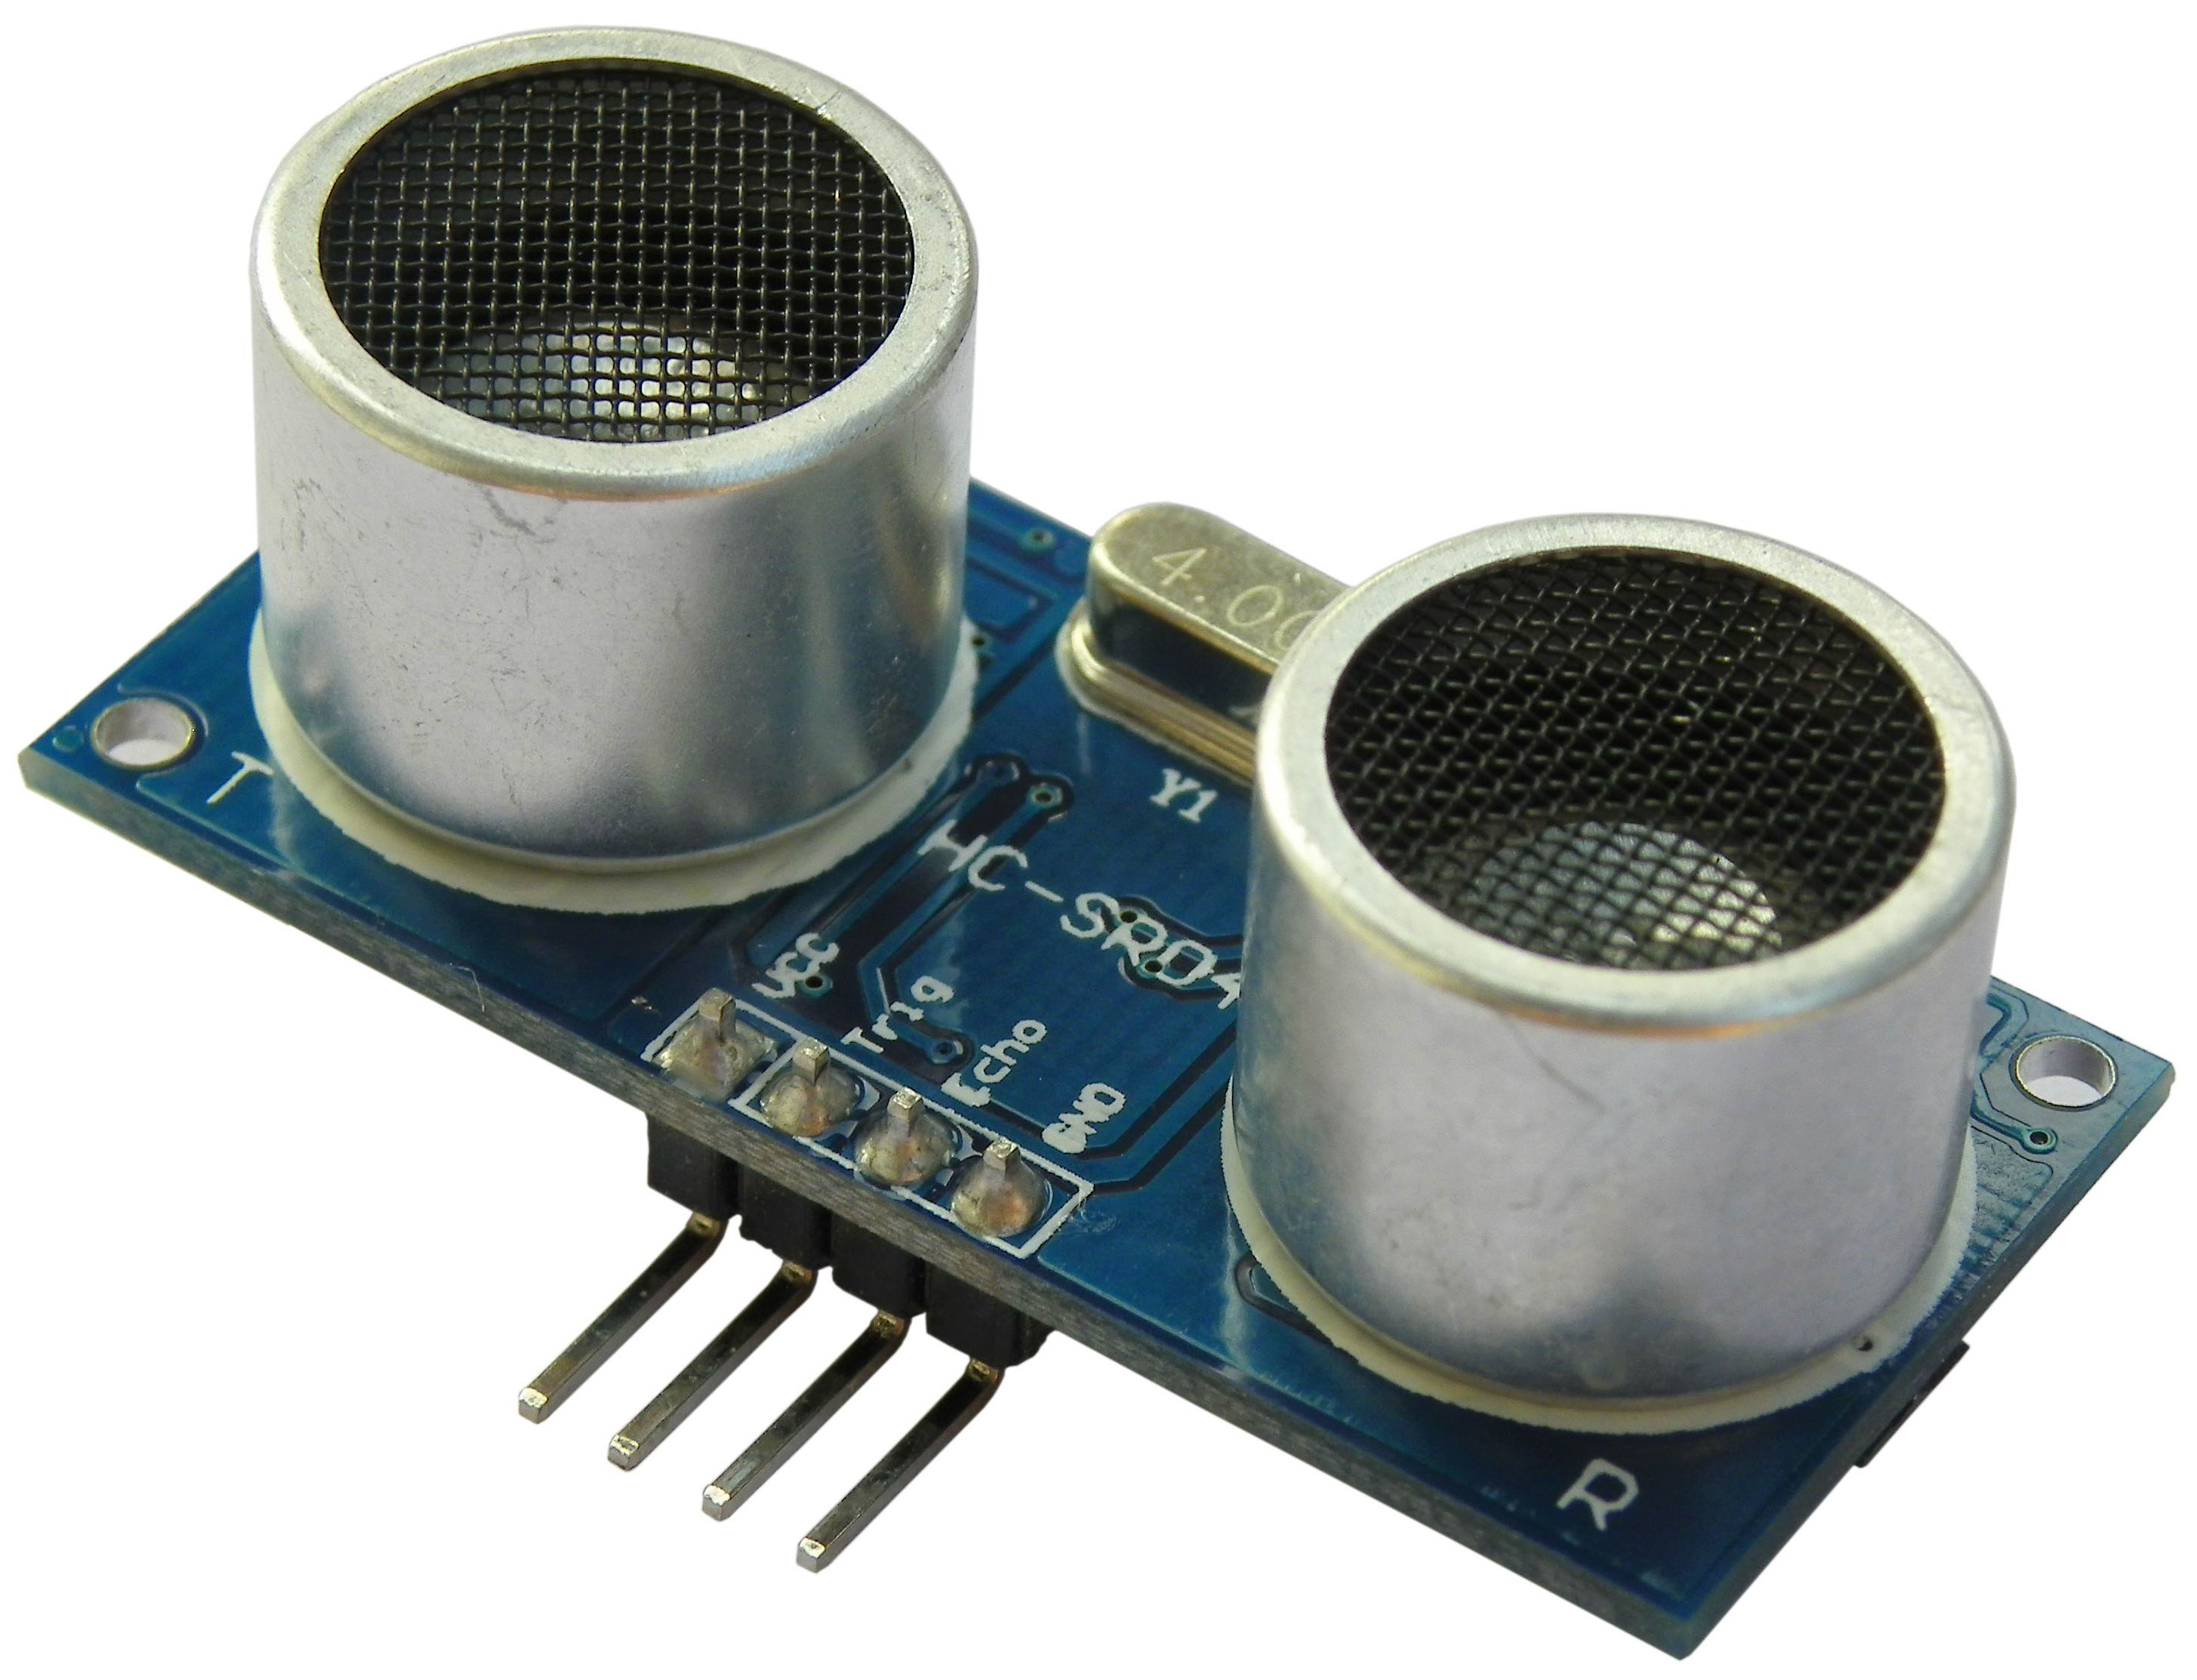
\includegraphics[width=2in]{HC-SR04-lg.jpg}
\caption{HC-SR04 ultrasonic sensor}
\end{figure}

\begin{figure}[ht]
\centering
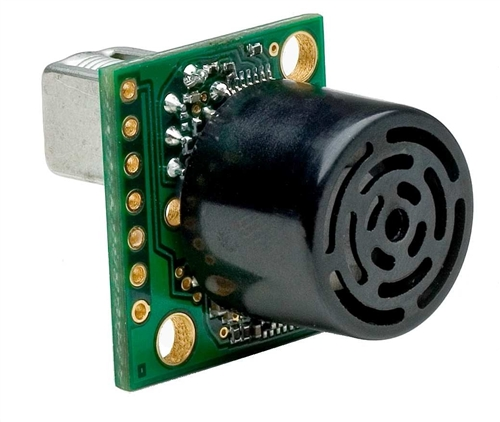
\includegraphics[width=2in]{ultrasonic.jpg}
\caption{An ultrasonic sensor available from AndyMark}
\end{figure}

\section{Beam}
\begin{figure}[ht]
\centering
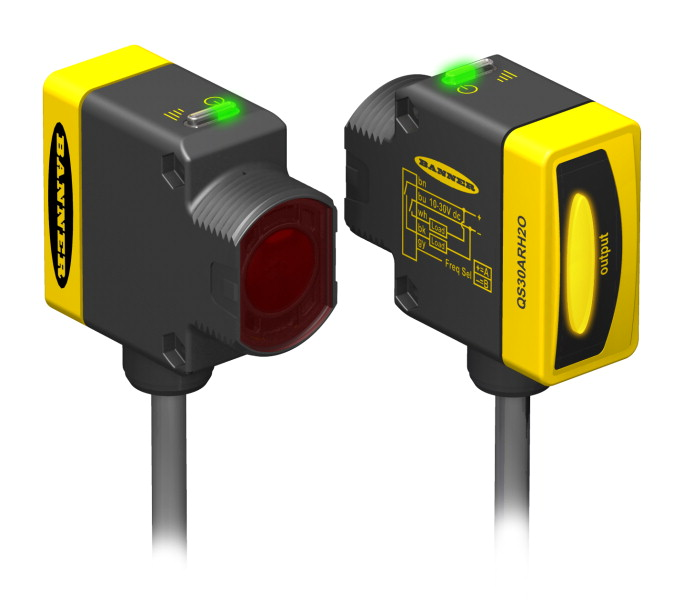
\includegraphics[width=2in]{beam.jpeg}
\caption{This Banner-brand beam sensor is designed for detecting the presence of fluids}
\end{figure}

\section{IR Sensor}
\begin{figure}[ht]
\centering
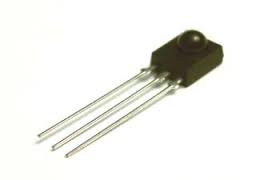
\includegraphics[width=2in]{ir_sensor.jpeg}
\caption{An IR sensor}
\end{figure}
with beacon/transmitter

\section{IR rangefinder}
\begin{figure}[ht]
\centering
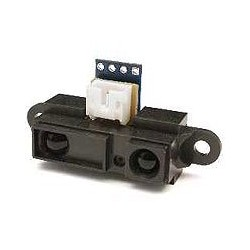
\includegraphics[width=2in]{ir-rangefinder.jpg}
\caption{Sharp-brand analog IR rangefinder}
\end{figure}

analog type
digital type
surfaces
\section{Light sensor}
		-skirts
\section{Compass}

Compass sensors are exactly what they sound like: A compass with an electronic readout.  They work by measuring magnetic fields.  are available and some teams have used them.  However, likely to be held in buildings made out of steel-reinforced concrete
\section{Camera}
computer vision
stereo vision
\section{Integrated processing camera}
 (cost)
\section{Lidar}
\begin{figure}[ht]
\centering
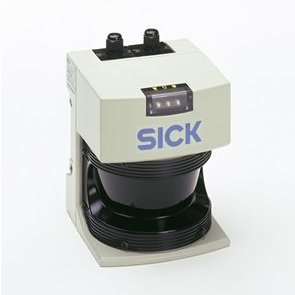
\includegraphics[width=2in]{SICK_LMS291.jpg}
\caption{A SICK LMS291 Lidar (circa 2004)}
\end{figure}

Lidar sends laser pulses in many directions so that the locations of objects can be inferred.  I don't know of any FRC team that has even attempted to use Lidar.  There are several reasons for this:
\begin{itemize}
\item There are FRC rules about lasers and most (and it used to be all) Lidar sensors run afoul of them.  
\item Most Lidar units exceed the cost limits.  Historically, the lowest-end models would still be in the thousands of dollars although costs have come down.  
\item A high level of programming effort is required.  
\end{itemize}

%xbox's sensor with camera \& depth information Kinect

%\section{RADAR}

\section{GPS}
GPS is not used on FRC robots for two reasons: 1) events are held indoors and the reception would be terrible and 2) doing so would violate the rules about devices that send and receive signals.

\section{IMU}
fancy ones not used (cost)
\section{Microphones}
- too noisy/not efficient

\end{document}
